\section{Our proposal: Hybrid DE for the FJSSP}
\label{sec:HDE}
\vspace{-0.2cm}
In this section, our proposal to solve the  FJSSP is detailed. In order to apply the DE algorithm, it is crucial to design a suitable encoding scheme that maps the floating point vectors to the feasible solution for the FJSSP (see Section~\ref{subsec:rep}). Moreover, our proposal is enhanced by a simple local search (Section~\ref{subsec:HDE}). Finally, a parallel version of our proposal is introduced (Section~\ref{subsec:parallelHDE}).


\subsection{Representation}  \label{subsec:rep}
\vspace{-0.25cm}
In this work, the DE algorithm still manipulates real-valued vector in order to maintain the simplicity and properties of the DE in their natural configuration. Consequently, the schedule is generated following the random keys encoding scheme~\cite{Bean1994RepRandomKeys}. This representation deals with real point vectors, where these points are used as sort keys to decode the solution. For an $n$-job $m$-machine scheduling problem, each vector's position (a random key) consists of a floating number in U(-1,1) which can be translated to an unique list of ordered operations, after a descending order of the random keys. These steps always obtain a feasible schedule from a real-valued vector. The schedule is a permutation with repetitions~\cite{bierwirth1995}. See Figure~\ref{fig:decodificacion} for an example considering the instance shown in Table~\ref{tab:proccesingTime}. Given the vector $x_i^g$=[0.6,-0.5,0.4,-0.3,-0.1,0.9,-0.7,0.2], it is converted to a schedule $[2, 1, 1, 3, 2, 2, 1, 3]$, which is a permutation of the set of operations that represents a tentative ordering to schedule them, each one being represented by its job number. This valid schedule corresponds to the operation sequence $O_{21}$, $O_{11}$, $O_{12}$, $O_{31}$, $O_{22}$, $O_{23}$, $O_{13}$, and $O_{32}$. 

In order to evaluate $x_i^g$, the objective value is the makespan ($C_{max}$). To compute it, each operation $O_{ij}$ in $x_i^g$ is assigned to a feasible machine $M_k$ in $U_{ij}$ with the shortest completion time, and then the load of $M_k$ must be updated. The initial solution is generated by a random procedure (Equation 1), mainly because high performing construction heuristics for the FJSSP are unknown.
%
%The decoding procedure is explained in Algorithm~\ref{alg:algoritmoDecodificacion} and is applied before the evaluation of an vector begins. An illustrative example is shown in FigureXX.
%
%En la figura \ref{fig:decodificacion} se puede ver un ejemplo de este procedimiento para una instancia del problema FJSSP con 3 trabajos, 4 máquinas y 8 operaciones mostrada en la tabla
%
\begin{figure}[tb]
    \centering
    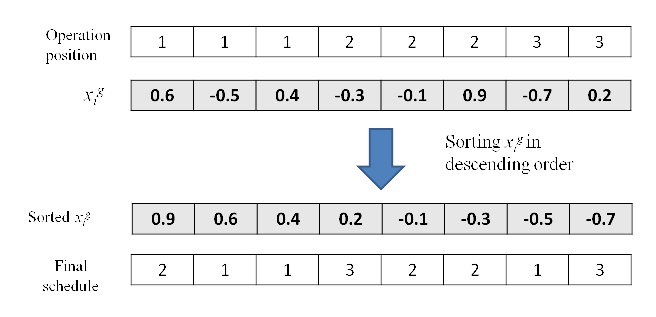
\includegraphics[width=0.55\textwidth]{./figures/deco.eps}
    \caption{Example of the decoding process used by the DE to solve the FJSSP.}
    \label{fig:decodificacion}
    \vspace{-0.4cm}
\end{figure}
%
\subsection{DE and Local Search Method} \label{subsec:HDE}
\vspace{-0.25cm}
DE is enhanced with a local search technique, yielding a hybrid DE (HDE) for exploration and exploitation among the solutions to obtain a near optimal solution. In this work, a simple interchange mechanism is implemented in which two positions of the target vector are randomly selected  and interchanged. If there is an improvement in the objective function the swap is accepted, otherwise, it is not considered. %The pseudo-code of local search procedure is given in Figure~\ref{alg:algoritmoLS}. 
This local search procedure is applied to the target vectors $x_{i}$ of the next population (just before Line 11 of Algorithm~\ref{alg:algoritmoDE}) but not to the trial vector $u_{i}$, which is beneficial to avoid both cycling search and getting trapped in a local optimum. Moreover, the frequency of the local search is controlled by the probability $p_{LS}$. Another important characteristic of this local search procedure is that it does not need a backward conversion because it is applied over the real-valued vector.
%
%
%Con el fin de mejorar la eficiencia de DE, se incorporó al algoritmo un procedimiento de busqueda local, que actua sobre la población justo antes de la línea 10 del algoritmo \ref{alg:algoritmoDE}. En el algoritmo \ref{alg:algoritmoLS} se puede ver un pseudocodigo del proceso realizado, el cual consiste en iterar sobre todos los individuos de la población, obtener un número aleatorio y si es menor a una probabilidad de aplicar busqueda local realizar las siguientes acciones: seleccionar 2 indices aleatorios en el individuo $x_{i}$, intercambiar entre ellos obteniendo un nuevo vector de prueba $u_{i}$, y si al evaluar $u_{i}$ obtenemos una solución igual o mejor que $x_{i}$, seleccionar $u_{i}$ como nuevo individuo de nuestra población.
%
%\begin{algorithm} [H]
%    \caption{Local Search Procedure} \label{alg:algoritmoLS} 
%    \begin{algorithmic} [1]
%        \For {each $x_{i}^g$ from $P^{g}$}
%            \If {$random() < PBL$} %\Comment PBL: probabilidad de busqueda local
%                \State $j$ , $k \leftarrow $ random(1,$D$)
%                \State $u_{i} \leftarrow $ swap($x_{i}$, $j$,$k$)
%                \If {$f(u_{i}) \leq  f(x_{i})$} \Comment{for a minimization problem}
%                    \State $x_{i} \leftarrow u_{i}$
%                \EndIf
%            \EndIf
%        \EndFor
%    \end{algorithmic}
%\end{algorithm}

\subsection{DE and Parallelism} \label{subsec:parallelHDE}
\vspace{-0.2cm}
In terms of designing parallel metaheuristics, the DE can be paralleled in different ways~\cite{Talbi}. %For instance, their population-based characteristics allow evaluating in a parallel way the fitness value of each individual, giving rise a global or master-slave model. In this same line, each iteration of a metaheuristic can be parallelized. In this two cases, the behaviour of the metaheuristic is not altered. Parallelism can also be exploited to perform the genetic operators in a semi-isolated manner, resulting in the island model. Finally, the previous strategies can be combined, giving rise to the cellular model~\cite{albaPEA2006}. This last two models alter the behavior of the metaheuristic and enable the improvement of the quality of solutions.
In this work, the aim of the parallelization is not to change the behaviour of the metaheuristic but to speed up the search. For that purposes, we focus on the parallelization of each iteration of the DE~\cite{albaPEA2006}. The population of individuals is decomposed and handled in parallel, using the well-known global parallelization model. A principal process performs the selection operations and the replacement, which are generally sequential. The rest processes (workers) perform the mutation, recombination, and the evaluation of the solutions in parallel. Consequently, this model maintains the sequence of the original algorithm, and hence the behavior of the metaheuristic is not altered. 








%Actuando sobre la eficiencia del algoritmo, con el fin de mejorar la velocidad del mismo, se optó por un esquema de ejecución en paralelo. Teniendo en cuenta que a cada individuo se lo trata por separado en el proceso de evolución, se cosideró realizar estas ejecuciones en paralelo, tomando cantidades iguales de individuos de la poblacion y asignando cada parte a unidades de procesamiento diferentes. La misma idea se tomo para mejorar la eficiencia en la búsqueda local, otorgando grandes ventajas en cuanto a velocidad y aprovechamiento de recursos.

%\subsection{Implementación de \textit{DE} híbrido para \textit{FJSSP}}
%El algoritmo \ref{alg:algoritmoDEhibrido} presenta el pseudocodigo del algoritmo de \textit{DE} hibrido para \textit{FJSSP}. Como se puede observar el esquema general es el mismo que el presentado anteriormente, con la inclusión del proceso de búsqueda local. Además, se agrega como entrada la probabilidad de aplicar busqueda local ($PBL$).

%\begin{algorithm} [H]
%    \caption{Pseudocodigo de la Evolucion Diferencial (DE)} \label{alg:algoritmoDEhibrido}
%    \begin{algorithmic} [1]
%    \Require {$F, Cr, N_p, PBL$} 
%    \Ensure {$x_{best}$} 
%        \State inicializar($P$,$N_p$) 
%        \State $g \leftarrow 0$
%        \While {no se alcance la condición de fin}
%            \For {cada vector $x_{i}^g$ de $P^g$}
%                \State $v_{i}^g \leftarrow $ mutacion($x_{i}^g, P^g, F$) 
%                \State $u_{i}^g \leftarrow $ recombinacion($x_{i}^g, v_{i}^g, Cr$)
%                \State $x_{i}^g \leftarrow $ seleccion($x_{i}^g, u_{i}^g$)
%                \State agregar($P^{g+1}, x_{i}^{g+1}$) 
%            \EndFor
%            \State busqueda-local($P^g$, $PBL$)
%            \State $g \leftarrow g+1$ 
%        \EndWhile
%        \State$x_{best} \leftarrow $mejor-solucion($P^{g}$)
%
%    \end{algorithmic}
%\end{algorithm}



